% !TeX root = ../protokoll.tex
% =====================================================================
%  AUSWERTUNG  (Abschnitt 1.4 der Anleitung)
%  Zuerst Originaldaten, dann alle daraus gewonnenen Ergebnisse.
%  Zu JEDEM berechneten Wert eine Fehlerbetrachtung;
%  Fehler als Fehlerbalken in Auftragungen kenntlich machen.
% =====================================================================
\section{Auswertung}
\label{cap:Auswertung}

\begin{comment}
    -erst Originaldaten, dann abgeleitete Werte
    -zu jedem Wert Fehlerbetrachtung
    -Fehlerbalken in beiden Achsrichtungen
\end{comment}

\subsection{Originaldaten}
\label{cap:Originaldaten}
Messwerte tabelliert; signifikante Stellen orientieren sich am niedrigst-signifikanten Messwert:
\begin{table}[H]
    \centering
    \caption{Beispiel-Messreihe mit statistischen Unsicherheiten}
    \begin{tabular}{c|c}
        \label{tab:Messreihe}
        $t$ in s & $s$ in mm \\
        \hline
        1.0 & 2.1 ± 0.2 \\
        2.0 & 4.3 ± 0.2 \\
        3.0 & 6.2 ± 0.3 \\
        4.0 & 8.5 ± 0.3 \\
    \end{tabular}
\end{table}

\subsection{Auftragung}
\label{cap:Auftragung}
Alle Achsen mit Einheiten beschriften; Einheiten so wählen, dass viele Nullen vermieden werden. Statistische Fehler der Datenpunkte in beide Richtungen als Fehlerbalken darstellen und in die Anpassung einfließen lassen:
\begin{figure}[H]
    \centering
    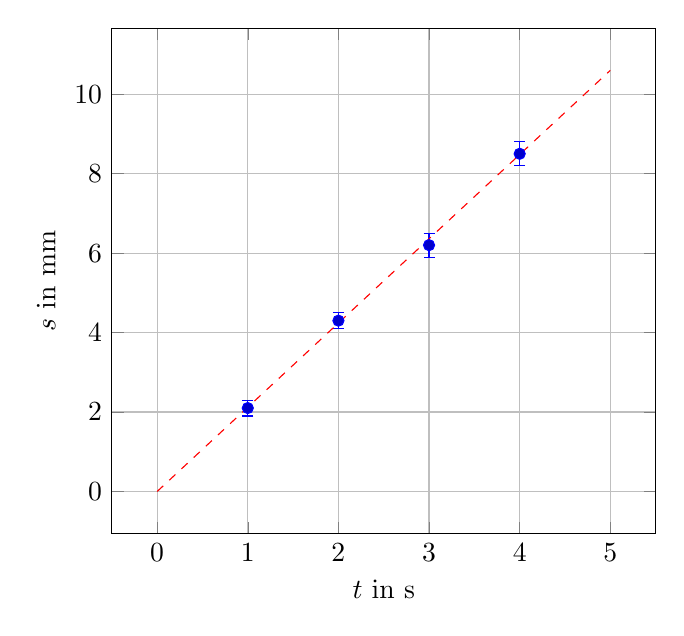
\begin{tikzpicture}
        \begin{axis}[
            width=0.7\textwidth,
            height=8cm,
            xlabel={$t$ in s},
            ylabel={$s$ in mm},
            grid=major,
        ]
            \addplot+[
                only marks,
                error bars/.cd,
                    x dir=both, x explicit,
                    y dir=both, y explicit,
            ] coordinates {
                (1.0, 2.1) +- (0.0, 0.2)
                (2.0, 4.3) +- (0.0, 0.2)
                (3.0, 6.2) +- (0.0, 0.3)
                (4.0, 8.5) +- (0.0, 0.3)
            };
            \addplot+[domain=0:5, dashed, no marks] {2.12*x};
        \end{axis}
    \end{tikzpicture}
    \caption{Messwerte mit statistischen Unsicherheiten als Fehlerbalken sowie lineare Ausgleichsgerade mit $v=(2.1\pm0.1)$\,mm/s}
    \label{fig:Fit}
\end{figure}

\subsection{Fehlerbetrachtung}
\label{cap:Fehlerbetrachtung}
Hier werden die Unsicherheiten der Messwerte, der Ausgleichung und der Ergebnisse über Gleichung \eqref{equ:Fehlerfortpflanzung} diskutiert. Beispiel für die Ergebnisnotation (Wert und Fehler in derselben Einheit, dieselbe Anzahl an Nachkommastellen, Fehler aufrunden):
\begin{align}
    v = (12.3 \pm 0.4)\,\mathrm{mm/s}
    \label{equ:Ergebnis}
\end{align}
